\section{SCG}
Flere metoder kan benyttes til at måle de vibrationer forårsaget af det kardiovaskulæresystem. Her kan f.eks. nævnes ballistocardiografi, mechanocardigram og seismocardiografi. Disse vibrationer indeholder information om den mekaniske funktion af det kardiovaskulære system. En metode der er blevet foreslået til at være et brugbart værktøj ift. detektering af begivenhederne i hjertets cyklus er SCG \cite{phd}. 

Kort beskrevet repræsenterer SCG-signalet de vibrationer i brystvæggen, der er forårsaget af hjertets sammentrækning og udstrømning af blod fra ventriklerne. Ved hjælp af  SCG kan den mekaniske aktivitet af hjertet måles, via vibrationer på brystvæggen. Disse vibrationer optages ofte med et enkelt akset eller 3-akset accelerometer, dog beskriver størstedelen af den fundne litteratur  brugen af et enkelt akset accelerometer der fokuserer på bevægelser i den dorso–ventrale retning \cite{Recent_Advances}.

\subsection{SCG-signalet}
Acceleration er den tidsafledede af hastigheden, altså tilvækst i hastighed pr. tidsenhed. Derfor giver SCG god information om hjertes bevægelser igennem dens cyklus \cite{performance}, dog  foreligger en variation i tolkningen af betydningen af de forskellige events i SCG-signalet \cite{phd}. Udfordringerne kommer af den komplekse bølgeform som er vanskelig at fortolke \cite{zanetti}, da der ikke er fuld forståelse for hvordan alle begivenheder i hjertecyklussen giver sig til kende på SCG-signalet, da bølgerne fra de enkelte begivenheder kan påvirke hinanden \cite{abra}.

Størstedelen af SCG signal befinder sig i området 4-50 [Hz], hvoraf hovedparten af signalet vil ligge under 20 [Hz] i de fleste tilfælde \cite{phd}. 
SCG målt på ældre mennesker viser en lavere signal amplitude i forhold til raske unge mennesker \cite{Recent_Advances}. Placering af måleinstrumentet er ligeledes af stor betydning, da signaler er direkte påvirket af placeringen af SCG sensoren \cite{zanetti}. SCG vil desuden oftest måles sammen med EKG for at kunne aflæse de samlede elektromekaniske egenskaber for hjertet \cite{abra}. De forskellige begivenheder er illustreret på figur \ref{fig:wigger}.


\begin{figure}[H] % Example of including images
\begin{center}
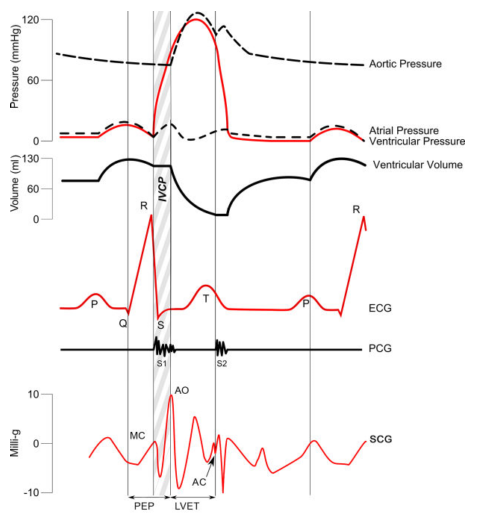
\includegraphics[width=1\textwidth]{figures/wigger}
\end{center}
\caption{De forskellige begivenheder i SCG signalet \cite{zanetti}.}
\label{fig:wigger}
\end{figure}

\newpage
\subsection{Anvendelse af SCG}
SCG har været foreslået til klinisk brug på en række områder. Blandt andet har SCG været foreslået til at kunne tilnærme sig myocardielle kontraktilitet udtrykt ved $dP/dt_{max}$ (maksimum afledte af tryk). Den nuværende guldstandard for måling af samme parameter foregår ved benyttelse af et kateter, hvor trykket i venstre ventrikel måles. SCG har også været foreslået til at estimere hjertets slagvolumen. Slagvolumen er en indikator for den myocardiale kontraktilitet og har en tæt korrelation til $dP/dt_{max}$.SCG er også blevet foreslået til måle begivenhederne i de systoliske og diastoliske tidsintervaller for at estimere ydeevnen for den venstre ventrikel. Her kan nævnes  præ-ejektions perioden (PEP) og venstre ventrikulær ejektions tid (LVET) som kan udrages af SCG-signalet, hvilket også kan ses på figur \ref{fig:wigger} \╬cite{zanetti}. 

Forlænget PEP og forkortet LVET er relateret til reduceret slagvolumen og cardiac output. Desuden er det blevet vist at PEP forkortes når kontraktiliteten stiger, hvilket f.eks. kan benyttes som præ-screening af patienter med synkroniseringsproblemer i hjertet   Af andre anvendelser af SCG kan f.eks. nævnes diagnose og monitering af koronararteriesygdom og måling af heart rate varibilty \cite{zanetti}  \cite{abra}.

I majoriteten af studier omhandlende SCG, fokuseres der ofte på at optage informationer der relaterer sig til det kardiovaskulære system. Flere studier har foreslået at SCG er velegnet til at udtrække informationer om respiration. Et studiet fandt at start-eksspiration og peak-eksspiration kunne udledes fra SCG signalet \cite{pandia} \cite{magic}. Denne information vil  bl.a. kunne bruges til at detektere abnormaliteter i respirationsmønster ved søvnforstyrrelser \cite{tavaloka}. Respiration kan påvirke signalet ved enten at påvirke SCG signalets baseline, ændre amplituden af bølgerne i SCG-signalet og ændring i RRI (low-frequency power of R-R interval). Hvor meget man kan aflæse ud fra de enkelte parametre er dog meget individuelt \cite{magic}.

 SCG er af ikke invasiv karakter, hvorfor påmontering i eget hjem med lethed ville kunne implementeres, hvad enten der er tales om patches eller straps til påmontering. Et studie af \cite{Wearable} har implementeret et accelerometer i en tætsiddende trøje for lettere at kunne forbinde patienten til sensoren. Med let tilgængelighed samt håndterbarheden af moderne accelerometre \todo{giv eksempel på den model vi benytter} er der muligheder for monitorering af SCG enheder på patienter i hjemmet, med telemedicinsk opkobling til hospitalet. Dermed kan et screeningssystem der anvender SCG til hjemmemonitorering muligvis være fordelagtigt i forbindelse med hjerteudredningen der anvendes i dag.
